\documentclass[11pt]{article}
\usepackage[margin=1in]{geometry}
\usepackage{mathtools,amssymb,amsthm,booktabs,tabularx,enumitem}
\usepackage[hidelinks]{hyperref}
\usepackage{parskip}
\usepackage{algorithm}
\usepackage{algpseudocode}
\usepackage{graphicx}
\usepackage{float}
\usepackage{caption}
\usepackage{xcolor}
\newcommand{\tie}[1]{\textcolor{red}{#1}}
\setlist{nosep}
\DeclareMathOperator*{\argmax}{arg\,max}
\DeclareMathOperator*{\argmin}{arg\,min}
\DeclareMathOperator{\dist}{dist}
\newcommand{\pos}[1]{[#1]_+}
\newcommand{\tbd}{-}
\theoremstyle{definition}
\newtheorem{definition}{Definition}
\newtheorem{assumption}{Assumption}
\theoremstyle{plain}
\newtheorem{proposition}{Proposition}

\title{Persistent Patrolling and Severity-Scaled Emergency Response\\
for Heterogeneous Ground-Air Robot Teams\\[4pt]
\large Final skeleton (internal)}
\author{}
\date{17 November 2026}

\begin{document}
\maketitle
\vspace{-2em}

\noindent\textbf{What this document is.} The sieved, internal version of
the working formulation (the dump document). It keeps only
the model, the method, the algorithms, the evaluation design and the
results. Every result is shown as - until we run it on our own copy of
the code. The only numbers left
are settings and stated bounds.

\section{Overview}

We extend Time-Period-Based Patrolling (TPBP) from a team of ground robots
to a team of ground robots (UGVs) and aerial robots (UAVs) on a road
network that also contains \emph{air-only} locations, which no UGV can
reach. UGVs patrol the roads with the TPBP walk-selection rule. UAVs ride
on UGVs, launch to air-only locations when a carrier passes close by, and
land on a UGV again at a coordinated meeting point. Emergency events
temporarily take a severity-dependent number of robots off patrol.

\begin{table}[H]
\centering
\small
\caption{Relation to TPBP.}
\label{tab:new}
\begin{tabularx}{\linewidth}{lX}
\toprule
Status & Mechanism \\
\midrule
Unchanged & Priority nodes, time period $T$, valid-walk definition, the four-term walk reward, claim set of destination priority nodes. \\
Changed & Overlap discount in the reward (Sec.~\ref{sec:select}); continuous occupancy in idleness (Sec.~\ref{sec:idle}). \\
New & Air-only nodes; starvation guard; ghost credit; recovery credit; UAV launch, cap, landing candidates and rendezvous; severity quota and responder selection; covering walk set (Sec.~\ref{sec:cover}). \\
\bottomrule
\end{tabularx}
\end{table}

\section{Notation}

\begin{table}[H]
\centering
\small
\caption{Symbols. Times are in seconds, distances in metres.}
\label{tab:notation}
\begin{tabularx}{\linewidth}{lX}
\toprule
Symbol & Meaning \\
\midrule
\multicolumn{2}{l}{\textit{Graph and time}} \\
$G = (V, E)$ & Operating graph: node set $V$, undirected edge set $E$. \\
$V_g$, $V_a$ & Ground (road) nodes and air-only (``ghost'') nodes; $V = V_g \cup V_a$, disjoint. \\
$S \subseteq V_g$ & Priority nodes. $s, f$ denote priority nodes. \\
$w(u, v)$ & Travel time of edge $(u,v)$ for a UGV: edge length divided by $v_g$. \\
$v_g$, $s_a$ & UGV speed and UAV speed. \\
$d(u, v)$ & Shortest UGV travel time from $u$ to $v$ on $G$. \\
$d(v, S)$ & $\min_{s \in S} d(v, s)$: travel time from $v$ to its nearest priority node. \\
$q_v$ & Planar position of node $v$. \\
$T$ & Time period shared by all priority nodes (TPBP). \\
$T_h$ & $T$ in hops on a uniform grid: $T$ divided by the hop time. \\
$H$ & Evaluation horizon. \\
\multicolumn{2}{l}{\textit{Idleness and objective}} \\
$I_v(t)$ & Idleness of node $v$ at time $t$: time since the last visit. \\
$t_v^{\mathrm{last}}$ & Time of the last visit to $v$. \\
$\pos{x}$ & $\max(x, 0)$. \\
$J$ & Objective: time-averaged node idleness plus priority overshoot. \\
\multicolumn{2}{l}{\textit{Walks and walk selection}} \\
$p$ & A walk $(v_0, \ldots, v_m)$; $v_0 = s_o$ is its start, $v_m = s_f$ its end. \\
$V(p)$ & Set of distinct nodes of $p$. \\
$L(p)$ & Number of nodes of $p$. \\
$T_p$ & Travel time of $p$: $\sum_{i} w(v_i, v_{i+1})$. \\
$\mathcal{P}$ & Stored set of candidate walks, built offline. \\
$\mathcal{P}_o(t)$ & Walks in $\mathcal{P}$ that start at the deciding UGV's node and end in $Y(t)$. \\
$X(t)$, $Y(t)$ & Destinations of the other UGVs' current walks; $Y(t) = S \setminus X(t)$. \\
$\dist(p, s)$ & $\min_{v \in V(p)} d(v, s)$: distance from walk $p$ to priority node $s$. \\
$R(p, t)$ & Reward of walk $p$ at time $t$. \\
$c_1, \ldots, c_4$ & TPBP reward weights: idleness, overshoot, distance, length. \\
$O_g(t)$ & Nodes on the remaining walks of all UGVs other than $g$. \\
$\omega_v(t)$, $\delta$ & Overlap weight of node $v$ and overlap discount. \\
$\tau_s = \kappa_s T$ & Starvation threshold for road nodes. \\
\bottomrule
\end{tabularx}
\end{table}

\begin{table}[H]
\centering
\small
\caption*{Symbols (continued).}
\begin{tabularx}{\linewidth}{lX}
\toprule
Symbol & Meaning \\
\midrule
\multicolumn{2}{l}{\textit{UAV service}} \\
$h$ & An air-only node; $q_h$ its position. \\
$r_{\max}$ & Launch radius. \\
$L_h$ & Launch set of $h$: ground nodes within $r_{\max}$ of $q_h$. \\
$x_g(t)$ & Position of UGV $g$ at time $t$, including mid-edge. \\
$Q^-$ & Claim set: air-only nodes that a launched UAV is heading to or servicing. \\
$c_5, c_6$ & Ghost-credit weights. \\
$I_{\min}$ & Minimum idleness of $h$ before it can earn ghost credit. \\
$c_7$ & Recovery-credit weight. \\
$\hat t_{\mathrm{rem}}(h)$ & Remaining service time at an occupied air-only node $h$. \\
$\tau_a = \kappa_a T$ & Air-only idleness cap. \\
$\ell_u$ & Remaining planned path length of UGV $u$. \\
$C$ & Number of landing candidates per UGV. \\
$t_u(u, r)$ & UGV $u$'s travel time to landing point $r$. \\
$t_a(h, r)$ & UAV flight time from $h$ to $r$: $\|q_r - q_h\| / s_a$. \\
$T_L$, $t_{\mathrm{dep}}$ & Earliest joint arrival time at a landing point; UAV departure delay. \\
$\varepsilon_\ell$ & Docking tolerance. \\
\multicolumn{2}{l}{\textit{Events}} \\
$e_v(t)$ & Event flag at node $v$. \\
$\sigma$ & Event severity, $\sigma \in \{1, 2, 3\}$. \\
$q_g(\sigma)$, $q_a(\sigma)$ & UGV and UAV responder quotas. \\
$\mathcal{G}_e$, $\mathcal{A}_e$ & Eligible UGVs and UAVs at the time of the event. \\
\multicolumn{2}{l}{\textit{Covering walk set}} \\
$T^\star$ & Smallest $T$ at which every edge lies on a valid walk. \\
$\pi(v)$ & Owner of $v$: the priority node nearest $v$. \\
$G_S$, $D_S$ & Graph on $S$ linking pairs at most $T$ apart; its largest hop distance. \\
$U$ & Off-path nodes: ground nodes on no direct walk. \\
$C_{sf}$ & Corridor of pair $(s, f)$: nodes $v$ with $d(s,v) + d(v,f) \leq T$. \\
$m$ & Walks kept from each priority node through each launch set. \\
$U^\dagger$ & Off-path nodes that lie only on gated detours. \\
$p_v$, $s_v$ & A stored walk through $v$, and its start. \\
$N_c$ & Most UGVs holding a starvation claim at once. \\
$d$ & Maximum node degree of $G$. \\
$w_{\min}$ & Travel time of the shortest edge. \\
$n_{\max}$ & Largest number of edges in a valid walk: $\lceil T / w_{\min} \rceil$. \\
\bottomrule
\end{tabularx}
\end{table}

\section{Problem Formulation}

\subsection{Graph}

The environment is an undirected graph $G = (V, E)$ with $V = V_g \cup
V_a$. Ground nodes $V_g$ are road intersections, connected by the edges
$E$; both robot types can visit them. Air-only nodes $V_a$ have no edges;
only a UAV, flying directly, can visit them. A node is air-only because it
has no road access, not by label. The priority nodes $S \subseteq V_g$ are
as in TPBP; air-only nodes are not priority nodes.

\begin{assumption}[Flight]
A UAV flies in a straight line at constant speed $s_a$ without obstacles.
Flight dynamics, collisions and battery limits are not modelled.
\end{assumption}

\begin{assumption}[Charging]
Docking recharges a UAV instantly.
\end{assumption}

\subsection{Idleness}
\label{sec:idle}

The idleness of node $v$ at time $t$ is
\begin{equation}
I_v(t) = t - t_v^{\mathrm{last}},
\end{equation}
the time since any robot last visited $v$. A visit resets it to zero.

\begin{definition}[Continuous occupancy]
While a robot stays at a node to service it, the node's idleness is held at
zero for the whole stay, not only at the instant of arrival. This covers a
UAV servicing an air-only node and a robot waiting at a meeting point for
the other robot.
\end{definition}

\subsection{Objective}

\begin{equation}
J = \frac{1}{H} \int_0^H \Bigg[ \frac{1}{|V|} \sum_{v \in V} I_v(t)
+ \frac{1}{|S|} \sum_{s \in S} \pos{I_s(t) - T} \Bigg] dt .
\label{eq:J}
\end{equation}
The first term is the mean idleness over all nodes, ground and air-only.
The second is the priority overshoot: zero while every priority node is
revisited within $T$, positive once a revisit is late. The horizon $H$ and
the event schedule are fixed by the evaluation protocol.

In the results we report \emph{combined idleness}: mean road idleness plus
mean air-only idleness, each averaged over the horizon. It weighs the two
node classes equally regardless of their sizes; it is not $J$.

\section{Routine Patrolling}

\subsection{Valid walks}

\begin{definition}[Valid walk]
A valid walk $p = (v_0, \ldots, v_m)$ starts and ends at priority nodes,
$v_0 = s_o \in S$ and $v_m = s_f \in S$, possibly $s_o = s_f$, and takes at
most the time period: $T_p \leq T$.
\end{definition}

The definition is TPBP's. TPBP stores a set $\mathcal{P}$ of valid walks,
computed once offline. Which walks to store is a design choice; we
use the covering set of Section~\ref{sec:cover}, and all results of
Section~\ref{sec:results} use it. The \emph{old} set, used in earlier
versions and reported for comparison, held for each ordered priority pair
the 500 walks with the fewest hops, plus the walks $s \to v \to f$
(shortest path from $s$ to $v$, then from $v$ to $f$) for every ground node
$v$, all filtered to $T_p \leq T$. Air-only
nodes are never on a walk; only UAVs reach them.

\subsection{Walk selection}
\label{sec:select}

When UGV $g$ finishes its walk it picks the next one,
\begin{equation}
p^\star = \argmax_{p \in \mathcal{P}_o(t)} R(p, t),
\end{equation}
over the stored walks that start at its node and end at a priority node no
other UGV is heading to ($Y(t)$). The reward is TPBP's, with the overlap
weight $\omega_v$ added:
\begin{equation}
R(p, t) = c_1 \sum_{v \in V(p)} \omega_v(t)\, I_v(t)
+ c_2 \sum_{s \in V(p) \cap Y(t)} \pos{I_s(t) - T}
- c_3 \sum_{s \in Y(t)} \dist(p, s)
- c_4\, L(p) .
\label{eq:R}
\end{equation}
Term 1 rewards visiting stale nodes; term 2 rewards visiting overdue
priority nodes; term 3 penalises walks that end far from the unclaimed
priority nodes; term 4 penalises length.

\paragraph{Overlap discount.} With $\omega_v = 1$ (TPBP), a UGV is rewarded
for a stale node that another UGV is already heading to, so larger fleets
crowd the same roads. We set
\begin{equation}
\omega_v(t) = \begin{cases} 1 - \delta, & v \in O_g(t), \\ 1, &
\text{otherwise,} \end{cases} \qquad 0 \leq \delta \leq 1,
\end{equation}
where $O_g(t)$ is the set of nodes on the remaining walks of the other
UGVs. $\delta = 0$ recovers TPBP. Overlap is discouraged, not forbidden.

\paragraph{Starvation guard.} Because the reward sums idleness over a walk,
a node that only short walks reach can lose to long walks for hours. If
some road node has $I_v(t) > \tau_s = \kappa_s T$, take the stalest such
node that some walk in $\mathcal{P}_o(t)$ covers, and restrict the argmax to
the walks that cover it. This restricts the candidate set; it does not
change $R$. The guard and the overlap discount apply to every variant,
including the UGV-only floor. With the covering walk set, off-path nodes
are also served by gated detours and claims (Section~\ref{sec:claim}).

\subsection{Ghost credit}
\label{sec:ghost}

Equation~\eqref{eq:R} has no reason to bring a UGV near an air-only node.
A UGV carrying a launch-ready UAV therefore adds to $R(p, t)$
\begin{equation}
c_5 \left( I_h(t) + c_6 \pos{I_h(t) - T_p} \right)
\label{eq:ghost}
\end{equation}
for the first air-only node $h$ (in a fixed order) such that
(i) $p$ passes through the launch set $L_h = \{ v \in V_g : \|q_v - q_h\|
\leq r_{\max} \}$,
(ii) the UGV carries a docked, launch-ready UAV,
(iii) $I_h(t) \geq I_{\min}$, and
(iv) $h \notin Q^-$.
The first part rewards a stale air-only node; the second adds a bonus once
$h$ has been idle longer than the walk takes. At most one air-only node is
credited per walk. The credit only steers walk choice; the launch itself is
decided by Section~\ref{sec:launch}.

\subsection{Recovery credit}
\label{sec:rec}

A UAV that finishes service needs a free UGV nearby. A UGV that is
\emph{free} (no docked UAV, not reserved) adds to $R(p, t)$
\begin{equation}
\frac{c_7}{\hat t_{\mathrm{rem}}(h)}
\end{equation}
for the first air-only node $h$ that is being serviced by a UAV and whose
launch set $p$ passes through. $\hat t_{\mathrm{rem}}(h)$ is the remaining
service time, floored at $0.1$\,s, so the pull grows as service nears its
end. A node is either unclaimed (ghost credit may apply) or being serviced
(recovery credit may apply), never both.

\section{UAV Service Cycle}

\subsection{Carrying}
Each UAV rides docked on a UGV, at most one per UGV, whenever it is not
servicing an air-only node.

\subsection{Launch}
\label{sec:launch}

At every time step, including mid-edge, a UGV $g$ carrying a launch-ready
UAV launches it to
\begin{equation}
h^\star = \argmin_{h \notin Q^-,\ \|x_g(t) - q_h\| \leq r_{\max}}
\|x_g(t) - q_h\| ,
\end{equation}
the nearest unclaimed air-only node within $r_{\max}$, with ties broken by
higher $I_h(t)$. $h^\star$ is added to $Q^-$. No launch site and no target
is fixed in advance.

\paragraph{Air-only idleness cap.} If no unclaimed air-only node is within
$r_{\max}$ but some unclaimed $h$ has $I_h(t) > \tau_a = \kappa_a T$, the
UAV launches to the stalest such node, provided its carrier is within
$r_{\mathrm{rec}}$ of it (the same bound as the recovery flight) and no
other docked UAV is closer to it. This bounds the worst air-only idleness at
about $\tau_a$ plus the time for a carrier to come within $r_{\mathrm{rec}}$.
It applies only to variants that launch by proximity.

\subsection{Service and recovery}
\label{sec:cycle}

\begin{enumerate}
\item \textbf{Service.} The UAV flies to $h^\star$; $I_{h^\star}$ is held at
zero while it stays.
\item \textbf{Recovery assignment.} The candidates are the free UGVs whose
current position is within the recovery radius $r_{\mathrm{rec}} = 500$\,m of $h^\star$
(straight line, $\|x_u(t) - q_{h^\star}\| \leq r_{\mathrm{rec}}$). For each candidate $u$ with remaining planned path length $\ell_u$, the landing
points are the nodes of that path at distances $\ell_u/3$, $2\ell_u/3$ and
$\ell_u$ (each snapped to the first path node at or beyond it; duplicates
merged), so at most $C = 3$ points; a landing point $r$ is kept only if
$\|q_r - q_{h^\star}\| \leq r_{\mathrm{rec}}$. For landing point $r$,
\begin{equation}
T_L(u, r) = \max\big( t_u(u, r),\ t_a(h^\star, r) \big), \qquad
t_{\mathrm{dep}} = T_L - t_a(h^\star, r),
\end{equation}
where $T_L$ is the earliest time both robots can be at $r$ and
$t_{\mathrm{dep}}$ is how long the UAV keeps servicing before it leaves.
The pair $(g^\star, r^\star) = \argmin_{u, r} T_L(u, r)$ is chosen and
$g^\star$ is reserved: it cannot be picked by another UAV or as an event
responder. If no UGV and landing point lie within $r_{\mathrm{rec}}$, the UAV keeps
servicing $h^\star$ (its idleness stays at zero) and tries again at the next
step. Every recovery flight is therefore at most $r_{\mathrm{rec}}$ long.
\item \textbf{Rendezvous.} The UAV stays at $h^\star$ until
$t_{\mathrm{dep}}$, then flies to $r^\star$. $g^\star$ continues its walk to
$r^\star$. Whichever arrives first waits, holding $r^\star$ at zero
idleness. Write $W_a$ and $W_g$ for the UAV's and the UGV's waiting time.
\item \textbf{Docking.} When both are within $\varepsilon_\ell$ the UAV
docks and recharges, $h^\star$ leaves $Q^-$, $g^\star$ is released, and
both resume.
\end{enumerate}

\section{Emergency Events}

\label{sec:events}
\subsection{Event model}
An event sets $e_v(t) = 1$ at any node $v$ (ground, priority or air-only)
and carries a severity $\sigma \in \{1, \ldots, \sigma_{\max}\}$,
$\sigma_{\max} = 3$. An event at an air-only node can only be answered by a
UAV. A response is mandatory: every slot of the quota is filled, at onset
or as soon as a robot becomes available. Responders travel to $v$ (UGV by
shortest path, UAV by direct flight). While a responder travels it is
still on the graph, so the nodes it passes are visited as usual. While at
least one responder is at $v$, the node is held at idleness 0
(Definition~1, continuous occupancy). The baseline protocol injects one
event per run.

\emph{Work rule.} An event of severity $\sigma$ needs
$W(\sigma) = (q_g + q_a)\, h_e$ robot-seconds of work at $v$, with
$h_e = T$. Every responder on site does one robot-second per second, so
a full team clears it in $h_e$ once on site, and a short team takes
proportionally longer. $\tau_{\mathrm{clear}}$ is the time from onset to
the moment the work is done.

\emph{After clearing.} Each responding UGV drives to its nearest priority
node and resumes walk selection there. Each responding UAV starts a normal
recovery from $v$ (Section~\ref{sec:cycle}), so it lands on a UGV within
$r_{\mathrm{rec}}$ by the usual rule.

\subsection{Severity quota}
The quota scales with severity against a reference team of
$n_g^{\mathrm{ref}} = 2$ UGVs and $n_a^{\mathrm{ref}} = 2$ UAVs, the team
a worst-case event needs:
\begin{equation}
q_g(\sigma) = \left\lceil n_g^{\mathrm{ref}} \frac{\sigma - 1}{\sigma_{\max} - 1} \right\rceil,
\qquad
q_a(\sigma) = \left\lceil n_a^{\mathrm{ref}} \frac{\sigma - 1}{\sigma_{\max} - 1} \right\rceil,
\end{equation}
with at least one responder. At an air-only node $q_g = 0$ and
$q_a \geq 1$. The reference team is a property of the event, not of the
fleet: the same event takes the same robots from a large fleet as from a
small one.

\begin{table}[H]
\centering
\small
\caption{Responder quota $(q_g, q_a)$ and work $W$ by severity,
$n^{\mathrm{ref}} = 2/2$, $\sigma_{\max} = 3$, $h_e = T$.}
\label{tab:quota}
\begin{tabular}{cccc}
\toprule
Severity $\sigma$ & Ground node & Air-only node & Work $W$ (ground) \\
\midrule
1 & (1, 0) & (0, 1) & $1\,T$ \\
2 & (1, 1) & (0, 1) & $2\,T$ \\
3 & (2, 2) & (0, 2) & $4\,T$ \\
\bottomrule
\end{tabular}
\end{table}

\subsection{Eligibility and selection}

A UAV in a service cycle and a UGV reserved for a rendezvous are not
eligible. A UGV carrying a UAV (\emph{occupied}) that responds takes its
UAV along, filling one UGV slot and one UAV slot in one trip. A docked UAV
may fly to the event only if its carrier is within $r_{\mathrm{rec}}$ of
$v$, the same bound as the recovery flight. Selection
(Algorithm~\ref{alg:respond}): first send the nearest occupied UGVs, up to
$\min(q_g, q_a)$; then fill the remaining UGV quota with the nearest other
UGVs (by travel time); then fill the remaining UAV quota with the nearest
eligible UAVs (by flight distance).

\emph{Open slots.} A slot that cannot be filled at onset stays open and is
filled by the same rules as soon as a robot becomes eligible: a UGV is
released from its reservation, or a UAV lands. If a UAV slot is open and no
docked UAV is within $r_{\mathrm{rec}}$, the occupied UGV that can bring
its UAV within $r_{\mathrm{rec}}$ soonest drives toward $v$ (a
\emph{courier}); its UAV takes off as soon as it is in range, and the
courier resumes patrolling.

\section{Covering Walk Set}
\label{sec:cover}

\textbf{Status:} implemented and evaluated on M1 and M3 (Section~\ref{sec:results}).

\subsection{Why the stored set matters}

The definition of a valid walk fixes \emph{which} walks are allowed; it
does not fix which of them are stored. TPBP stores all of them
\cite{mallya2021}. Let $d$ be the maximum node degree, $w_{\min}$ the
travel time of the shortest edge, and
\begin{equation}
n_{\max} = \left\lceil T / w_{\min} \right\rceil
\end{equation}
the largest number of edges a valid walk can have. TPBP's offline step
extends walks edge by edge from each priority node and keeps every walk
that can still reach a priority node within $T$; walks may revisit nodes.
Mallya et al.\ bound the result themselves \cite{mallya2021}: at most
$d^{\,n_{\max}}$ valid walks start at any priority node, so
\begin{equation}
|\mathcal{P}_{\mathrm{TPBP}}| \;\leq\; |S|\, d^{\,n_{\max}} ,
\end{equation}
exponential in $n_{\max}$. Their experiments use maps of at most 25 nodes
and walks of at most 12 edges, with about 2\,s per walk assignment. Two
things push $n_{\max}$ up on real maps. First, a large map needs a large
$T$ or many priority nodes (Proposition~\ref{prop:cover}). Second, on a
road network a single short edge sets $w_{\min}$: on M3 the shortest edge
is 2\,m, so $w_{\min} = 0.5$\,s and $n_{\max} = 800$ at $T = 400$\,s.
The old set capped the count at 500 walks per pair plus detours, at most
$500|S|^2 + |S|^2|V_g|$ walks, but a cap gives no guarantee that a given
node is on any walk from a given start, and on M3 it held 83\,054 walks.

The TPBP paper lists two open directions \cite{mallya2021}: bounds on the
feasible values of $T$, and a less data-intensive strategy than storing all
valid walks. Proposition~\ref{prop:cover} and the choice of $T$ below give
the first. The covering set below addresses the second: it still stores
walks, but linearly many in the map size instead of exponentially many in
$n_{\max}$.

\subsection{Which nodes can be covered}

\begin{proposition}
\label{prop:cover}
A ground node $v$ lies on some valid walk if and only if $2\, d(v, S) \leq
T$.
\end{proposition}
\begin{proof}
If $2\,d(v, S) \leq T$, let $s$ be the priority node nearest to $v$; the
closed walk $s \to v \to s$ along shortest paths takes $2\,d(v, s) \leq T$
and is valid. Conversely, any valid walk through $v$ from $s_o$ to $s_f$
takes at least $d(s_o, v) + d(v, s_f) \geq 2\, d(v, S)$, which must be at
most $T$.
\end{proof}

So every ground node must be within $T/2$ of some priority node. On an $M
\times N$ grid with unit hops, the nodes within $r$ hops of one node number
at most $2r^2 + 2r + 1$, so with $r = \lfloor T_h/2 \rfloor$:
\begin{equation}
|S| \;\geq\; \frac{MN}{2r^2 + 2r + 1}, \qquad
|\mathcal{P}| \;\geq\; \frac{MN}{T_h + 1} ,
\end{equation}
the second because one walk has at most $T_h + 1$ nodes. Both are lower
bounds. For M1 ($10 \times 10$, $T_h = 16$, $r = 8$) they give $|S| \geq 1$
(we use 6) and $|\mathcal{P}| \geq 6$. For $100 \times 100$ with $T_h =
16$ they give $|S| \geq 69$ and $|\mathcal{P}| \geq 589$; keeping $|S| = 6$
requires $2r^2 + 2r + 1 \geq 10^4 / 6$, that is $r \geq 29$ and $T_h \geq
58$.

\paragraph{Choosing $T$.} Proposition~\ref{prop:cover} is about nodes.
Walks also use the roads between nodes, and moving between priority nodes
needs those roads, so the exact condition is per edge.

\begin{proposition}
\label{prop:edge}
An edge $(u, w) \in E$ lies on some valid walk if and only if
\begin{equation}
d(u, S) + w(u, w) + d(w, S) \leq T .
\end{equation}
\end{proposition}
\begin{proof}
A valid walk from $s_o$ to $s_f$ that crosses the edge from $u$ to $w$
takes at least $d(s_o, u) + w(u, w) + d(w, s_f) \geq d(u, S) + w(u, w) +
d(w, S)$; crossing it from $w$ to $u$ gives the same bound. Conversely,
the walk from the priority node nearest $u$ to $u$, across the edge, and
on to the priority node nearest $w$ takes exactly this time.
\end{proof}

Define
\begin{equation}
T^\star = \max_{(u, w) \in E} \big( d(u, S) + w(u, w) + d(w, S) \big),
\end{equation}
the smallest $T$ at which every road segment lies on a valid walk. For any
neighbour $w$ of $v$, $d(v, S) \leq w(v, w) + d(w, S)$, so $T^\star \geq
2 \max_{v \in V_g} d(v, S)$: $T \geq T^\star$ also satisfies
Proposition~\ref{prop:cover} for every ground node, and every launch set
lies on some valid walk. $T^\star$ needs one Dijkstra search per priority
node and works on any graph, grid or road network. No method whose walks
start and end at priority nodes within $T$ can put every road segment on
a walk with $T < T^\star$.

Let $G_S$ be the graph on $S$ that links $s$ and $f$ when $d(s, f) \leq
T$: the pairs of priority nodes a UGV can move between with one walk. Let
$\pi(v)$ be the priority node nearest $v$, the \emph{owner} of $v$.

\begin{proposition}
\label{prop:conn}
If the road graph is connected and $T \geq T^\star$, then $G_S$ is
connected.
\end{proposition}
\begin{proof}
Take $s, f \in S$ and a road path $s = v_0, v_1, \ldots, v_k = f$, with
$\pi(s) = s$ and $\pi(f) = f$. For consecutive nodes,
\begin{equation*}
d\big(\pi(v_i), \pi(v_{i+1})\big) \leq d(v_i, S) + w(v_i, v_{i+1}) +
d(v_{i+1}, S) \leq T^\star \leq T ,
\end{equation*}
so $\pi(v_i)$ and $\pi(v_{i+1})$ are equal or linked in $G_S$. The
sequence $\pi(v_0), \ldots, \pi(v_k)$ is a path from $s$ to $f$ in $G_S$.
\end{proof}

So not every pair of priority nodes has to be within $T$ of each other;
UGVs chain walks through $G_S$.

The rule, for a task with priority nodes $S$ and time period $T$:
\begin{itemize}
\item if $T \geq T^\star$, keep $S$ and $T$;
\item otherwise, either raise $T$ to $T^\star$, if the task allows the
priority deadline to be relaxed, or keep $T$ and add the fewest extra
priority nodes that bring $T^\star$ down to $T$.
\end{itemize}
The fewest extra nodes are found by an integer program. Let $x_v \in \{0,
1\}$ mark $v$ as a priority node, $z_{uv} \in \{0, 1\}$ assign node $u$ to
priority node $v$, and $r_u \geq 0$ bound the distance from $u$ to the
priority node it is assigned to:
\begin{equation}
\begin{aligned}
\min \;& \textstyle\sum_{v \in V_g} x_v \\
\text{s.t. } & x_s = 1 && \forall s \in S, \\
& \textstyle\sum_{v} z_{uv} = 1,\quad z_{uv} \leq x_v && \forall u, v \in V_g, \\
& r_u \geq \textstyle\sum_{v} d(u, v)\, z_{uv} && \forall u \in V_g, \\
& r_u + w(u, w) + r_w \leq T && \forall (u, w) \in E .
\end{aligned}
\end{equation}
Since $r_u \geq d(u, S)$, the last constraint gives the condition of
Proposition~\ref{prop:edge} on every edge; conversely, any priority set
that meets it is feasible, by assigning every node to its nearest
priority node. So the program is exact. It is feasible whenever every edge
takes at most $T$, and has $|V_g|^2$ assignment variables. The added nodes
are ordinary priority nodes, and every method we compare uses the same
final $S$.

Raising $T$ is affordable only because of the covering set: the full TPBP
set grows exponentially in $n_{\max}$, whereas the covering set grows
linearly in the map size. The cost is a looser deadline on the priority
nodes, since the same $T$ sets the overshoot term of $J$ and $R$.

\subsection{Construction}

Algorithm~\ref{alg:cover}, with $T \geq T^\star$. For a pair $(s, f)$ let
\begin{equation}
C_{sf} = \{\, v \in V_g : d(s, v) + d(v, f) \leq T \,\}
\end{equation}
be its \emph{corridor}. Every node of every valid walk from $s$ to $f$ lies
in $C_{sf}$, since the walk must reach $v$ from $s$ and then $f$ from $v$.
\begin{enumerate}
\item \textbf{Distances.} One Dijkstra search by travel time from every
priority node, cut off at $T$, gives $d(s, \cdot)$, $d(\cdot, S)$, $\pi(\cdot)$
and the shortest paths to and from every priority node, in $O(|S|(|E| +
|V_g| \log |V_g|))$. This replaces all-pairs shortest paths ($O(|V_g|^2)$
memory).
\item \textbf{Direct walks.} For every ordered pair $(s, f)$ with $d(s, f)
\leq T$, $s = f$ included, the $|C_{sf}|$ non-empty walks from $s$ to $f$ with
the shortest travel time, ranked by time (not by hops), searched inside
$C_{sf}$. The search is exact because no valid $s \to f$ walk leaves
$C_{sf}$, and it stays local on large maps. The number of walks per pair is
set by the map: one per corridor node. UGVs use these walks to move between
priority nodes, and the reward chooses among them as in TPBP.
\item \textbf{Off-path nodes.} $U$ is the set of ground nodes on no direct
walk. Dead ends (tails) are the typical case: a walk between two priority
nodes enters a dead end only to come back out.
\item \textbf{Detours.} While some node of $U$ is uncovered, take the
uncovered $u$ with the largest $d(u, S)$. Start a walk at its owner
$\pi(u)$ along the shortest path to $u$. While time remains, extend it to
the uncovered node of $U$ that adds the most new nodes per extra second.
Close it at a priority node within the remaining time, preferring
$\pi(u)$. Mark its nodes covered. A tail is covered by one detour to its
tip. Detours are \emph{gated} (below).
\item \textbf{Air-only nodes.} For every $h \in V_a$ and every priority node
$s$, keep at least $m$ stored walks from $s$ through $L_h$: the walks
$s \to v \to f$ for $v \in L_h$ and $f \in S$, cheapest first. A UGV can
therefore reach every launch set from every priority node.
\item Remove duplicates.
\end{enumerate}

\begin{proposition}
\label{prop:covset}
If $T \geq T^\star$, every detour is valid and every ground node lies on a
stored walk.
\end{proposition}
\begin{proof}
A ground node on no direct walk is in $U$. Each round of step 4 covers at
least the chosen $u$. The walk $\pi(u) \to u \to \pi(u)$ takes $2\, d(u,
S) \leq T^\star \leq T$, so a valid closure always exists, and an extension
is accepted only if the walk can still close within $T$. The loop ends
only when $U$ is covered.
\end{proof}

\subsection{Gated detours and starvation claims}
\label{sec:claim}

Detours serve off-path nodes, which have no deadline, so they must not
compete with the priority-to-priority walks at every decision. A detour is
\emph{gated}: it is not a candidate in the argmax until one of its nodes has
idleness above the starvation threshold $\tau_s = \kappa_s T$. From then on,
any UGV standing at the detour's start may take it, and the starvation
guard of Section~\ref{sec:select} restricts the choice to walks that cover
the stale node. Nodes that lie on some ungated walk are handled by the
starvation guard alone, as before.

Proposition~\ref{prop:covset} puts every node on a stored walk; it does not
make a UGV stand at the right start. A detour from $\pi(u)$ is only a
candidate for a UGV at $\pi(u)$. Off-path nodes are therefore also served
by a \emph{claim}. Let $U^\dagger \subseteq U$ be the off-path nodes that lie
only on gated walks (not on an air-only walk of step 5), $p_v$ the fastest
stored walk through $v$ (a detour), and $s_v$ its start.
\begin{enumerate}
\item \textbf{Trigger.} When $v \in U^\dagger$ has $I_v(t) > \tau_s$ and is
on no claimed walk, $v$ joins a first-in, first-out queue.
\item \textbf{Claim.} While fewer than $N_c$ UGVs hold a claim, the node at
the head of the queue is claimed by the UGV that can reach $s_v$
earliest: the remaining time of its current walk plus $d$ from that walk's
end to $s_v$.
\item \textbf{Route.} The claimed UGV finishes its current walk, follows
the fastest stored ungated walks along a shortest path in $G_S$ to $s_v$,
runs $p_v$, and releases the claim. While it holds the claim it ignores
the restriction to $Y(t)$.
\item All other UGVs keep choosing by $\argmax R$.
\end{enumerate}
The cap is set by the map and the fleet, not tuned: the share of the fleet
that may hold a claim equals the share of nodes that only claims and gates
serve,
\begin{equation}
N_c = \Big\lceil n_{\mathrm{UGV}} \, |U^\dagger| / |V_g| \Big\rceil .
\end{equation}
It is 0 when every node lies on an ungated walk. The exemption from $Y(t)$
is needed: $Y(t)$ only spreads UGVs over destinations, and without the
exemption a claimed UGV is blocked whenever the end of its next hop, or
$s_v$ itself, is another UGV's destination.

\begin{proposition}
\label{prop:claim}
Assume the road graph is connected, $T \geq T^\star$, $N_c \geq 1$ and no
events. Once $v \in U^\dagger$ is claimed, it is visited within $(D_S + 2)\,
T$, where $D_S$ is the largest hop distance between two nodes of $G_S$. No
node of $U^\dagger$ has idleness that grows without bound.
\end{proposition}
\begin{proof}
The claimed UGV ends its current walk within $T$, at a priority node. By
Proposition~\ref{prop:conn}, $G_S$ is connected, so at most $D_S$ stored
direct walks, each of at most $T$ and each available because of the
exemption, bring it to $s_v$. Then $p_v$ takes at most $T$. So every claim
ends within $(D_S + 2)\, T$. The queue holds each node at most once, so it
has at most $|U^\dagger|$ entries, and $N_c$ claims are served at a time; a
queued node is claimed within $\lceil |U^\dagger| / N_c \rceil (D_S + 2)\,
T$.
\end{proof}

The bound covers off-path nodes only. Nodes on ungated walks rely on the
starvation guard, which has no such bound, and priority deadlines stay
soft, as in TPBP: the overshoot term rewards meeting them, but nothing
enforces it.

\paragraph{Size.} Step 2 adds at most $|C_{sf}| \leq |V_g|$ walks per pair
and step 4 at most $|U|$, so
\begin{equation}
|\mathcal{P}| \;\leq\; \sum_{(s, f)} |C_{sf}| + |U| + m|S||V_a| \;\leq\;
|S|^2 |V_g| + |V_g| + m|S||V_a| ,
\end{equation}
polynomial in the map size, against $|S|\,d^{\,n_{\max}}$ for the full TPBP
set. On large maps $|C_{sf}|$ is set by $T$, not by the map, so the size grows
with the number of priority pairs within $T$ of each other.

\paragraph{What does not change.} The reward, overlap discount, starvation
guard, credits, launch, recovery and event rules, and the weights. Selection
is still the argmax over stored walks from the UGV's node that end in
$Y(t)$; gating only decides when a detour is among them, and a claimed UGV
follows its claim route.

\section{Algorithms}

\begin{algorithm}[H]
\caption{Persistent patrolling (one time step)}
\label{alg:patrol}
\begin{algorithmic}[1]
\State update the claim queue; assign claims, at most $N_c$ held (Sec.~\ref{sec:claim})
\For{each UGV $g$}
  \If{an event selects $g$ (Alg.~\ref{alg:respond})}
    \State divert $g$ to the event node; \textbf{continue}
  \EndIf
  \If{$g$ carries a launch-ready UAV}
    \State $h^\star \gets$ nearest unclaimed $h$ within $r_{\max}$ of $x_g(t)$
    \State \textbf{if} none: $h^\star \gets$ stalest unclaimed $h$ with $I_h > \tau_a$,
      $\|x_g(t) - p_h\| \leq r_{\mathrm{rec}}$, no closer docked UAV
    \If{$h^\star$ exists} add $h^\star$ to $Q^-$; launch (Alg.~\ref{alg:cycle}) \EndIf
  \EndIf
  \If{$g$ has finished its walk}
    \If{$g$ holds a claim}
      \State $p^\star \gets$ next walk of its claim route, ignoring $Y(t)$
    \Else
      \State $p^\star \gets \argmax_{p \in \mathcal{P}_o(t)} R(p, t)$ with overlap discount, credits, starvation guard and opened gates
    \EndIf
    \State assign $p^\star$ to $g$
  \EndIf
  \State move $g$ one step; visit nodes reached
\EndFor
\For{each UAV in a service cycle} advance it one step (Alg.~\ref{alg:cycle}) \EndFor
\State update $I_v(t)$ for all $v$, with continuous occupancy
\end{algorithmic}
\end{algorithm}

\begin{algorithm}[H]
\caption{UAV service cycle}
\label{alg:cycle}
\begin{algorithmic}[1]
\State fly to $h^\star$; hold $I_{h^\star} = 0$ while there
\State candidates $\gets$ free UGVs, each with $\leq C$ landing points
\State $(g^\star, r^\star) \gets \argmin_{u, r} T_L(u, r)$; reserve $g^\star$
\State service until $t_{\mathrm{dep}}$; fly to $r^\star$
\State the first to arrive waits, holding $r^\star$ at zero idleness
\State dock; remove $h^\star$ from $Q^-$; release $g^\star$
\end{algorithmic}
\end{algorithm}

\begin{algorithm}[H]
\caption{Event responder selection}
\label{alg:respond}
\begin{algorithmic}[1]
\Require event node $v$, severity $\sigma$, quotas $q_g = q_g(\sigma)$, $q_a = q_a(\sigma)$
\State $\mathcal{G}_e \gets$ UGVs not reserved
\State $\mathcal{A}_e \gets$ docked UAVs whose carrier is within $r_{\mathrm{rec}}$ of $v$
\State $k \gets \min(q_g, q_a)$
\While{$k > 0$ and an occupied UGV is in $\mathcal{G}_e$}
  \State send the nearest occupied UGV with its UAV; $k, q_g, q_a \gets k-1, q_g-1, q_a-1$
\EndWhile
\While{$q_g > 0$ and a UGV is left in $\mathcal{G}_e$}
  \State send the nearest remaining UGV; $q_g \gets q_g - 1$
\EndWhile
\While{$q_a > 0$ and a UAV is left in $\mathcal{A}_e$}
  \State send the nearest remaining UAV; $q_a \gets q_a - 1$
\EndWhile
\While{$q_g + q_a > 0$ and the event is not cleared} \Comment{every step}
  \State fill open slots by the rules above as robots become eligible
  \If{$q_a > 0$, no eligible UAV, no courier for this slot}
    \State send the occupied UGV that brings its UAV within $r_{\mathrm{rec}}$ of $v$ soonest
  \EndIf
\EndWhile
\end{algorithmic}
\end{algorithm}

\begin{algorithm}[H]
\caption{Covering walk set (offline)}
\label{alg:cover}
\begin{algorithmic}[1]
\Require $G$, $S$, $T \geq T^\star$, $V_a$, $m$
\For{each $s \in S$} Dijkstra from $s$, cut off at $T$ \EndFor
\State $\mathcal{P} \gets \emptyset$
\For{each ordered pair $(s, f)$ with $d(s, f) \leq T$, $s = f$ included}
  \State $C_{sf} \gets \{ v : d(s, v) + d(v, f) \leq T \}$
  \State add the $|C_{sf}|$ fastest non-empty walks $s \to f$ inside $C_{sf}$
\EndFor
\State $U \gets V_g \setminus \bigcup_{p \in \mathcal{P}} V(p)$; $\mathcal{D} \gets \emptyset$
\While{$U \neq \emptyset$}
  \State $u \gets \argmax_{x \in U} d(x, S)$; $p \gets$ shortest path $\pi(u) \to u$
  \While{some $x \in U$ can be added with the walk still closable within $T$}
    \State extend $p$ to the $x$ with most new nodes per extra second
  \EndWhile
  \State close $p$ at a priority node within $T$, preferring $\pi(u)$
  \State $\mathcal{D} \gets \mathcal{D} \cup \{p\}$; $U \gets U \setminus V(p)$
\EndWhile
\For{each $h \in V_a$, $s \in S$} ensure $m$ walks $s \to v \to f$ with $v \in L_h$ \EndFor
\State remove duplicates; \Return $\mathcal{P} \cup \mathcal{D}$, with $\mathcal{D}$ gated
\end{algorithmic}
\end{algorithm}

\paragraph{Complexity per decision.} Scoring a walk costs $O(L(p) + |S| +
|V_a|)$: its nodes, its distance to each unclaimed priority node, and the
air-only nodes for the credits. A decision scores the walks of
$\mathcal{P}_o(t)$, so its cost is proportional to the stored walks per
start; this is where the covering set helps. $O_g(t)$ is built once per
decision, size at most $n_{\mathrm{UGV}} \cdot \max_p L(p)$. The launch
check is $O(|V_a|)$ per UGV per step; recovery assignment is
$O(C \cdot n_{\mathrm{UGV}})$ per cycle; responder selection is
$O(|\mathcal{G}_e| + |\mathcal{A}_e|)$ per event.

\section{Evaluation Design}

\subsection{Maps}
\label{sec:maps}
\begin{itemize}
\item \textbf{M1}: $10 \times 10$ grid, 100 nodes, 180 edges of 100\,m,
6 priority nodes, 5 air-only nodes.
\item \textbf{M3}: OpenStreetMap road network, 500\,m around a point in
Boston: 204 nodes, 291 edges (2--483\,m, mean 69\,m), 13 priority nodes, 9
air-only nodes.
\end{itemize}

\emph{Scope.} The air-only credit and the landing-point recovery act
through choices: which walk a UGV takes and where a UAV lands. They need a
road graph with alternative routes. Both maps have them: M1 has 81
independent cycles ($|E| - |V| + 1$) and M3, a real road network, has 88.
On a near-tree graph almost every walk is forced, so there is little for
the credits to choose between; such graphs are outside the scope of this
method.

\begin{figure}[H]
\centering
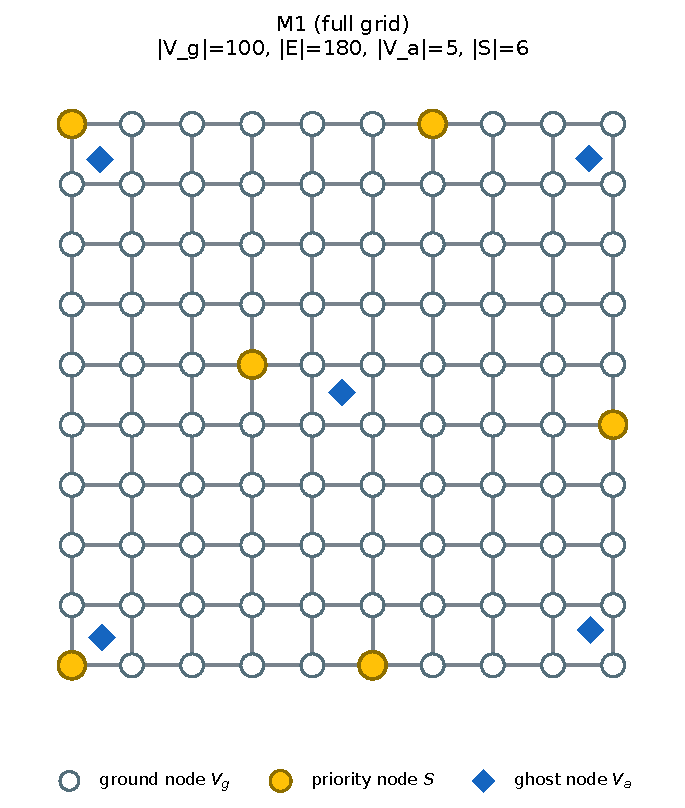
\includegraphics[width=0.45\linewidth]{sim/m1_map.pdf}
\caption{M1. Yellow: priority node. White: ground node. Blue diamond:
air-only node.}
\label{fig:m1}
\end{figure}

\begin{figure}[H]
\centering
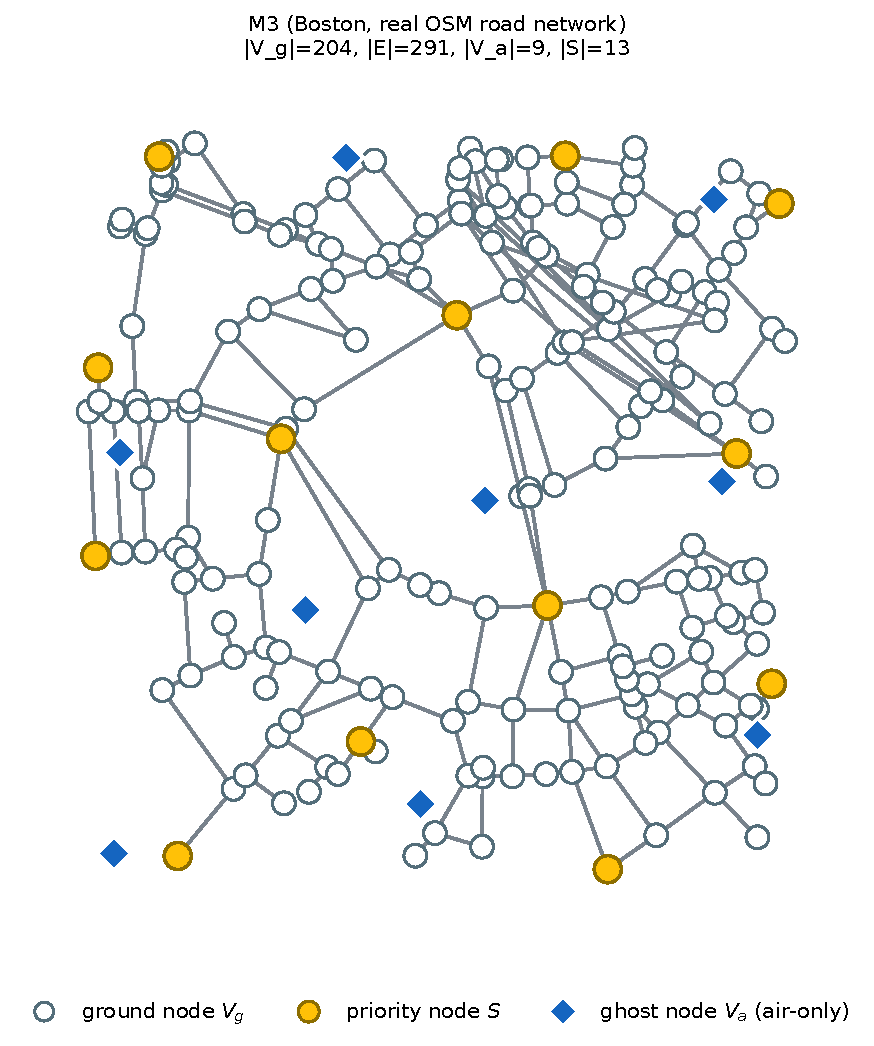
\includegraphics[width=0.6\linewidth]{sim/m3_map.pdf}
\caption{M3, the Boston road network. Same legend as
Figure~\ref{fig:m1}.}
\label{fig:m3}
\end{figure}

\subsection{Settings}
$v_g = 4$\,m/s (25\,s per 100\,m hop), $s_a = 12$\,m/s, $r_{\max} = 70$\,m
(launch), $r_{\mathrm{rec}} = 500$\,m (recovery, straight line), $\varepsilon_\ell = 2$\,m,
$C = 3$, 25\,s service dwell, $H = 2$\,h, $I_{\min} = 20$\,s, $\kappa_s = 4$,
$\kappa_a = 3$, $\delta = 0.5$, $m = 3$. Weights $c_1, \ldots, c_7 = 1, 2,
0.5, 0.1, 3, 1.5, 2$, untuned. Seeds 0--29 on both maps. On M3 the fleets 8/4, 10/5 and 10/7
are run. The event starts at $t_0 = H/2$, after the
patrol is in steady state, at a node drawn uniformly per seed over ground
and air-only nodes (the same node for every method and severity of that
seed).

\emph{Time period.} $T^\star$ is 200\,s on M1 and 420.2\,s on M3. By the
rule of Section~\ref{sec:cover}, M1 runs at $T = 400$\,s ($T_h = 16$;
$T \geq T^\star$, so $S$ and $T$ are kept), and M3 runs at $T = 421$\,s, the
first whole second above its $T^\star$.

\emph{Priority coverage.} The criteria of Section~\ref{sec:cover} are
enforced in the code: priority nodes are added until every ground node is
within $T/2$ of one and the edge criterion of Proposition~\ref{prop:edge}
holds. At the $T$ used, no node was added on M1; M3 meets the
criteria because $T \geq T^\star$.

\emph{Walk set.} All results use the covering walk set of
Section~\ref{sec:cover}. The \emph{old} walk set, used in earlier versions,
held the 500 fewest-hop walks per ordered priority pair plus the walks
$s \to v \to f$ through every node $v$, all filtered to $T_p \leq T$; it is
reported for comparison in Table~\ref{tab:cover}. Claim caps $N_c$: 0 on M1;
on M3 1 with 4, 6 or 8 UGVs and 2 with 10.

\subsection{Variants}
Each variant switches off exactly one mechanism of the full method.
\begin{itemize}
\item \textbf{V0, UGV-only (floor).} No UAVs. Shows road idleness of the
walk rule alone; air-only idleness grows without bound.
\item \textbf{V1, fixed launch nodes.} Launch only when a UGV stands on the
ground node nearest to $h$. No air-only cap.
\item \textbf{V2, no air-only credit.} $c_5 = 0$.
\item \textbf{V3, nearest-UGV recovery.} The UAV chases the nearest free
UGV's current position; no landing points, no waiting. The recovery
radius $r_{\mathrm{rec}}$ applies, and the chosen UGV stops until the UAV has landed on
it, so that the flight stays within the radius.
\item \textbf{V4, single responder.} Always send one nearest eligible
responder, whatever the severity. Same work $W(\sigma)$, so the lone
responder needs longer to clear a severe event.
\item \textbf{V5, random responders.} Fill the same quotas uniformly at
random among eligible robots.
\end{itemize}
V0 to V3 change the patrol and are compared with and without events; with
an event they all use Algorithm~\ref{alg:respond}. V0 has no UAVs, so it
cannot answer an event at an air-only node, and is left out of the event
tables. V4 and V5 change only the responder selection; the patrol is the
full method.

\subsection{Metrics}
Road idleness and air-only mean idleness $\bar I_a$ (both time-averaged),
their sum (combined), peak air-only idleness $I_a^{\max}$, peak road
idleness and peak priority idleness (worst value of any node in the run,
averaged over seeds). Variants are ranked on combined idleness. A margin
is the paired difference over seeds between the full method and the
baseline with the lowest mean; $t$ is the paired $t$ statistic ($|t| > 2.05$
is significant at 5\,\% with 30 seeds, 29 degrees of freedom). For events, each run with an
event is paired with the same seed's run without it (same method, fleet
and seed):
\begin{itemize}
\item $\Delta J_{\mathrm{event}}(\sigma)$: the rise in combined idleness
over the whole horizon, with the event against without it, in percent.
\item $\Delta J_{\mathrm{resp}}$: the same rise over the response only,
from onset to $\tau_{\mathrm{clear}}$.
\item $\Delta J_{\mathrm{post}}$: the same rise from
$\tau_{\mathrm{clear}} + T$ to the horizon, after the responders have had
one time period to rejoin the patrol.
\item $\tau_{\mathrm{clear}}$, the time from onset to clearing; first
arrival; $D_{\mathrm{resp}}$, the total responder travel distance;
shortfall, the quota slots not filled at onset.
\item \emph{Frozen check.} A run without the event in which, at the onset
time, the same quota of robots (chosen nearest first as in
Algorithm~\ref{alg:respond}) stops where it is for the measured
$\tau_{\mathrm{clear}}$, then resumes. The event run minus the frozen run
is the cost of the response beyond the loss of the robots it occupies.
\end{itemize}
For recovery: mean wait $\bar W$ over cycles of $W_a + W_g$.

\section{Results}
\label{sec:results}

Rows or cells in \tie{red} are those where the full method does not have the
lowest mean combined idleness. Bold marks the lowest combined idleness in
each block. All results are over seeds 0--29, and the margin tables give
the paired $t$ statistic ($|t| > 2.05$ is significant at 5\,\%).

\emph{Summary.} Over the 32 cells of M1 and M3 (fleet $\times$ no event
and $\sigma = 1, 2, 3$), the full method is never significantly worse than
any baseline. It is significantly better in 27: every cell of M3 and of
the M1 fleets with spare UGV capacity (4/2, 5/2, 6/3, and 5/1 except at
$\sigma = 3$). With 4 UGVs and 1 UAV, the smallest fleet that patrols M1,
it ties the best baseline in all four cells.

\subsection{M1, no events}

\begin{table}[H]
\centering
\small
\caption{M1, no event, covering walk set, 500\,m recovery radius, mean over seeds 0--29, 2-hour horizon, idleness in seconds.}
\label{tab:m1}
\begin{tabular}{llrrrrrr}
\toprule
Fleet & Variant & Road & Air mean & Air peak & Combined & Road peak & Prio.\ peak \\
\midrule
4 / 1 & full method & 408.5 & 627.4 & 2481.9 & \textbf{1035.8} & 1979.1 & 856.5 \\
 & no air-only credit & 403.1 & 640.2 & 2382.5 & 1043.3 & 1964.0 & 866.8 \\
 & fixed launch nodes & 411.2 & 1018.1 & 4296.4 & 1429.3 & 1987.5 & 869.0 \\
 & nearest-UGV recovery & 413.8 & 626.8 & 2297.7 & 1040.7 & 1977.6 & 863.9 \\
 & UGV-only (floor) & 403.2 & 3599.5 & 7199.0 & 4002.7 & 1947.6 & 861.1 \\
\addlinespace
4 / 2 & full method & 411.5 & 401.3 & 1545.3 & \textbf{812.8} & 2002.4 & 884.0 \\
 & no air-only credit & 404.9 & 431.7 & 1650.6 & 836.6 & 1978.8 & 861.4 \\
 & fixed launch nodes & 415.7 & 529.3 & 2440.1 & 944.9 & 2021.1 & 882.4 \\
 & nearest-UGV recovery & 423.9 & 430.7 & 1531.9 & 854.6 & 2074.5 & 901.6 \\
 & UGV-only (floor) & 403.2 & 3599.5 & 7199.0 & 4002.7 & 1947.6 & 861.1 \\
\addlinespace
5 / 1 & full method & 329.7 & 618.8 & 2517.8 & \textbf{948.6} & 1845.5 & 603.7 \\
 & no air-only credit & 326.4 & 662.5 & 2636.8 & 988.9 & 1806.2 & 603.1 \\
 & fixed launch nodes & 329.6 & 1017.4 & 4212.4 & 1347.0 & 1848.4 & 599.7 \\
 & nearest-UGV recovery & 335.5 & 672.7 & 2702.9 & 1008.2 & 1825.4 & 630.5 \\
 & UGV-only (floor) & 324.3 & 3599.5 & 7199.0 & 3923.8 & 1781.8 & 603.3 \\
\addlinespace
5 / 2 & full method & 332.7 & 404.2 & 1677.9 & \textbf{736.9} & 1860.1 & 604.7 \\
 & no air-only credit & 327.1 & 449.7 & 1702.7 & 776.8 & 1816.9 & 604.4 \\
 & fixed launch nodes & 333.4 & 533.7 & 2515.9 & 867.1 & 1842.2 & 611.1 \\
 & nearest-UGV recovery & 337.7 & 428.7 & 1650.3 & 766.4 & 1844.7 & 614.7 \\
 & UGV-only (floor) & 324.3 & 3599.5 & 7199.0 & 3923.8 & 1781.8 & 603.3 \\
\addlinespace
6 / 3 & full method & 267.7 & 343.7 & 1483.9 & \textbf{611.4} & 1688.7 & 365.7 \\
 & no air-only credit & 259.7 & 419.7 & 1493.8 & 679.4 & 1516.4 & 365.7 \\
 & fixed launch nodes & 266.8 & 1145.6 & 6324.2 & 1412.4 & 1609.9 & 365.7 \\
 & nearest-UGV recovery & 268.0 & 377.7 & 2122.6 & 645.7 & 1575.4 & 373.2 \\
 & UGV-only (floor) & 259.1 & 3599.5 & 7199.0 & 3858.6 & 1492.1 & 365.7 \\
\bottomrule
\end{tabular}
\end{table}

The full method has the lowest combined idleness in all five fleets. Its
margin over the closest baseline (Table~\ref{tab:m1evmargin}, first column)
is significant with 4/2 ($-23.9$\,s, $t = -4.83$), 5/1 ($-40.3$\,s,
$t = -3.28$), 5/2 ($-29.5$\,s, $t = -4.67$) and 6/3 ($-34.3$\,s,
$t = -5.23$), and not resolved with 4/1 ($-4.8$\,s, $t = -0.39$). Its
air-only mean is the lowest in four of five fleets (with 4/1 nearest-UGV
recovery is lower by 0.6\,s), and its road idleness is within 9\,s of the
lowest in every fleet. With 4 UGVs and 1 UAV the three variants that
launch by proximity are within 8\,s of each other. The four UGVs are the
fewest that patrol M1, so the walk bending and recovery reservations of the
credits cost road idleness (full: 408.5\,s against 403.1\,s for no air-only
credit), and a single UAV limits the air-only gain they buy (627.4\,s
against 640.2\,s); the two nearly cancel. With one more UGV (5/1) the same
single UAV gives a significant margin of 40.3\,s. The UGV-only floor cannot reach
air-only nodes, so its air-only idleness equals the horizon. Fixed launch
nodes is the weakest UAV variant in every fleet.

\subsection{M3, no events}

\begin{table}[H]
\centering
\small
\caption{M3 (Boston), no event, covering walk set, 500\,m recovery radius, $T = 421$\,s ($\geq T^\star$), mean over seeds 0--29, 2-hour horizon, idleness in seconds.}
\label{tab:m3}
\begin{tabular}{llrrrrrr}
\toprule
Fleet & Variant & Road & Air mean & Air peak & Combined & Road peak & Prio.\ peak \\
\midrule
8 / 4 & full method & 409.8 & 367.5 & 1561.8 & \textbf{777.3} & 3641.4 & 1100.1 \\
 & no air-only credit & 397.7 & 397.2 & 1566.5 & 794.9 & 3444.3 & 1112.3 \\
 & fixed launch nodes & 409.5 & 575.8 & 2922.6 & 985.3 & 3599.4 & 1153.8 \\
 & nearest-UGV recovery & 420.2 & 404.2 & 1646.8 & 824.4 & 3541.6 & 1154.0 \\
 & UGV-only (floor) & 398.9 & 3599.5 & 7199.0 & 3998.4 & 3653.3 & 1112.9 \\
\addlinespace
10 / 5 & full method & 366.9 & 331.2 & 1582.5 & \textbf{698.1} & 3589.4 & 1047.8 \\
 & no air-only credit & 359.2 & 360.8 & 1505.5 & 720.0 & 3569.4 & 973.8 \\
 & fixed launch nodes & 371.1 & 505.9 & 2876.0 & 877.0 & 3445.7 & 1085.0 \\
 & nearest-UGV recovery & 372.6 & 359.2 & 1539.8 & 731.8 & 3524.9 & 1068.1 \\
 & UGV-only (floor) & 357.9 & 3599.5 & 7199.0 & 3957.4 & 3594.0 & 1002.0 \\
\addlinespace
10 / 7 & full method & 366.3 & 255.4 & 1389.0 & \textbf{621.7} & 3516.3 & 1077.4 \\
 & no air-only credit & 357.2 & 291.5 & 1440.3 & 648.7 & 3764.2 & 1008.4 \\
 & fixed launch nodes & 369.8 & 340.2 & 1936.2 & 710.0 & 3475.8 & 1064.9 \\
 & nearest-UGV recovery & 372.0 & 279.5 & 1409.0 & 651.5 & 3688.8 & 1094.5 \\
 & UGV-only (floor) & 357.9 & 3599.5 & 7199.0 & 3957.4 & 3594.0 & 1002.0 \\
\bottomrule
\end{tabular}
\end{table}

The full method has the lowest combined idleness and the lowest air-only
mean in all three fleets; the margin over the closest baseline is
significant in all three (8/4: $-17.6$\,s, $t = -3.22$; 10/5: $-21.9$\,s,
$t = -4.68$; 10/7: $-27.0$\,s, $t = -5.80$; Table~\ref{tab:m3evmargin}).
The UGV-only rows for 10/5 and 10/7 are the same runs, since that variant
has no UAVs.

\subsection{M1 with events}
\label{sec:m1ev}

Table~\ref{tab:m1ev} runs every method on M1 without an event and with one
event of severity 1, 2 or 3. All methods answer the event with
Algorithm~\ref{alg:respond}; only the patrol differs.

\begin{table}[H]
\centering
\small
\caption{M1, combined idleness (s) over the whole 2-hour horizon, without an event and with one event at $t_0 = 3600$\,s, mean over seeds 0--29. In brackets: $\Delta J_{\mathrm{event}}$, the rise against the same method's run without the event. Bold: lowest in each column of a fleet.}
\label{tab:m1ev}
\begin{tabular}{llrrrr}
\toprule
Fleet & Method & No event & $\sigma = 1$ & $\sigma = 2$ & $\sigma = 3$ \\
\midrule
4 / 1 & full method & \textbf{1035.8} & \textbf{1042.9} (+0.7\,\%) & \tie{1080.2 (+4.3\,\%)} & \textbf{1121.9} (+8.3\,\%) \\
 & no air-only credit & 1043.3 & 1044.5 (+0.1\,\%) & \textbf{1077.5} (+3.3\,\%) & 1126.1 (+7.9\,\%) \\
 & fixed launch nodes & 1429.3 & 1419.0 ($-$0.7\,\%) & 1547.7 (+8.3\,\%) & 1588.7 (+11.2\,\%) \\
 & nearest-UGV recovery & 1040.7 & 1067.4 (+2.6\,\%) & 1097.1 (+5.4\,\%) & 1135.2 (+9.1\,\%) \\
\addlinespace
4 / 2 & full method & \textbf{812.8} & \textbf{819.0} (+0.8\,\%) & \textbf{831.0} (+2.2\,\%) & \textbf{866.9} (+6.7\,\%) \\
 & no air-only credit & 836.6 & 844.9 (+1.0\,\%) & 868.9 (+3.9\,\%) & 895.2 (+7.0\,\%) \\
 & fixed launch nodes & 944.9 & 943.8 ($-$0.1\,\%) & 967.3 (+2.4\,\%) & 1043.3 (+10.4\,\%) \\
 & nearest-UGV recovery & 854.6 & 858.0 (+0.4\,\%) & 871.9 (+2.0\,\%) & 895.9 (+4.8\,\%) \\
\addlinespace
5 / 1 & full method & \textbf{948.6} & \textbf{965.9} (+1.8\,\%) & \textbf{979.8} (+3.3\,\%) & \textbf{1030.1} (+8.6\,\%) \\
 & no air-only credit & 988.9 & 989.2 (+0.0\,\%) & 1047.1 (+5.9\,\%) & 1052.9 (+6.5\,\%) \\
 & fixed launch nodes & 1347.0 & 1356.2 (+0.7\,\%) & 1509.2 (+12.0\,\%) & 1527.4 (+13.4\,\%) \\
 & nearest-UGV recovery & 1008.2 & 1010.6 (+0.2\,\%) & 1035.4 (+2.7\,\%) & 1067.8 (+5.9\,\%) \\
\addlinespace
5 / 2 & full method & \textbf{736.9} & \textbf{735.6} ($-$0.2\,\%) & \textbf{745.8} (+1.2\,\%) & \textbf{782.7} (+6.2\,\%) \\
 & no air-only credit & 776.8 & 785.0 (+1.1\,\%) & 793.5 (+2.1\,\%) & 819.0 (+5.4\,\%) \\
 & fixed launch nodes & 867.1 & 880.5 (+1.5\,\%) & 907.5 (+4.7\,\%) & 963.6 (+11.1\,\%) \\
 & nearest-UGV recovery & 766.4 & 777.4 (+1.4\,\%) & 785.9 (+2.5\,\%) & 815.8 (+6.5\,\%) \\
\addlinespace
6 / 3 & full method & \textbf{611.4} & \textbf{612.0} (+0.1\,\%) & \textbf{621.0} (+1.6\,\%) & \textbf{626.8} (+2.5\,\%) \\
 & no air-only credit & 679.4 & 678.8 ($-$0.1\,\%) & 681.3 (+0.3\,\%) & 695.3 (+2.4\,\%) \\
 & fixed launch nodes & 1412.4 & 990.7 ($-$29.9\,\%) & 986.7 ($-$30.1\,\%) & 1015.1 ($-$28.1\,\%) \\
 & nearest-UGV recovery & 645.7 & 640.9 ($-$0.7\,\%) & 643.0 ($-$0.4\,\%) & 661.1 (+2.4\,\%) \\
\bottomrule
\end{tabular}
\end{table}

\begin{table}[H]
\centering
\small
\caption{M1, margin of the full method over the closest baseline (paired over seeds 0--29): difference in combined idleness (s), $t$ in brackets, and the number of seeds where the full method is lower. Negative: the full method is lower. $|t| > 2.05$ is significant at 5\,\%.}
\label{tab:m1evmargin}
\begin{tabular}{lrrrr}
\toprule
Fleet & No event & $\sigma = 1$ & $\sigma = 2$ & $\sigma = 3$ \\
\midrule
4 / 1 & $-4.8$ ($-0.39$) 16 & $-1.6$ ($-0.16$) 19 & \tie{$+2.7$ ($0.26$) 16} & $-4.1$ ($-0.34$) 18 \\
4 / 2 & $-23.9$ ($-4.83$) 26 & $-25.9$ ($-5.01$) 23 & $-37.9$ ($-5.88$) 25 & $-28.3$ ($-3.94$) 23 \\
5 / 1 & $-40.3$ ($-3.28$) 21 & $-23.3$ ($-2.14$) 18 & $-55.6$ ($-4.05$) 24 & $-22.8$ ($-1.36$) 18 \\
5 / 2 & $-29.5$ ($-4.67$) 23 & $-41.7$ ($-6.49$) 27 & $-40.1$ ($-5.80$) 26 & $-33.2$ ($-3.90$) 24 \\
6 / 3 & $-34.3$ ($-5.23$) 28 & $-28.9$ ($-5.13$) 25 & $-21.9$ ($-6.05$) 25 & $-34.3$ ($-8.01$) 28 \\
\bottomrule
\end{tabular}
\end{table}

The full method has the lowest combined idleness in 19 of the 20 cells, and
the margin is significant in 15 (all cells of 4/2, 5/2 and 6/3, and 5/1
without an event and at $\sigma = 1, 2$). With 5/1 at $\sigma = 3$ it is
lower by 22.8\,s, not resolved ($t = -1.36$). With 4/1 the three methods
with proximity launch tie in every column: the full method is lower by 1.6
to 4.8\,s in three cells and higher by 2.7\,s at $\sigma = 2$ ($t = 0.26$,
red); none of the four differences is resolved. Over the whole horizon the
event raises the full method's idleness by $-0.2$ to 1.8\,\% at
$\sigma = 1$, 1.2 to 4.3\,\% at $\sigma = 2$ and 2.5 to 8.6\,\% at
$\sigma = 3$, where a ground event takes two UGVs and two UAVs off patrol.
The rise is smallest with the largest fleet (6/3: at most 2.5\,\%), and the
baselines lose about as much, so the event does not change the ranking.
Fixed launch nodes with 6/3 is lower with the event than without it
(1412.4 to 990.7); its run without an event is far above its 4/2 and 5/2
values, and the event appears to move its UAVs out of a poor pattern. This
was not investigated further.

\begin{table}[H]
\centering
\small
\caption{M1, frozen check, full method: event run minus frozen run (same seed, same quota stopped for the same $\tau_{\mathrm{clear}}$), mean over seeds 0--29, $t$ in brackets. Response: combined idleness from onset to $\tau_{\mathrm{clear}}$, relative to the frozen run. Whole run: difference in combined idleness over the horizon (s).}
\label{tab:m1frozen}
\setlength{\tabcolsep}{3pt}
\begin{tabular}{lrrrrrr}
\toprule
& \multicolumn{3}{c}{Response window} & \multicolumn{3}{c}{Whole run} \\
Fleet & $\sigma = 1$ & $\sigma = 2$ & $\sigma = 3$ & $\sigma = 1$ & $\sigma = 2$ & $\sigma = 3$ \\
\midrule
4 / 1 & $-0.8$\,\% ($-0.83$) & $-1.7$\,\% ($-7.27$) & $-3.2$\,\% ($-10.42$) & $-9.2$ ($-1.14$) & $-8.7$ ($-0.86$) & $-3.2$ ($-0.37$) \\
4 / 2 & $-2.6$\,\% ($-4.38$) & $-4.3$\,\% ($-6.31$) & $-4.1$\,\% ($-10.22$) & $-5.1$ ($-1.31$) & $-3.0$ ($-0.60$) & $+7.1$ ($1.42$) \\
5 / 1 & $-2.6$\,\% ($-3.85$) & $-2.0$\,\% ($-6.41$) & $-3.2$\,\% ($-8.88$) & $-8.1$ ($-0.84$) & $-9.8$ ($-1.24$) & $+16.2$ ($2.01$) \\
5 / 2 & $-4.9$\,\% ($-2.79$) & $-4.7$\,\% ($-3.53$) & $-4.4$\,\% ($-8.33$) & $-8.4$ ($-1.92$) & $-8.1$ ($-2.21$) & $+1.5$ ($0.32$) \\
6 / 3 & $-2.2$\,\% ($-1.67$) & $-5.8$\,\% ($-4.77$) & $-6.9$\,\% ($-5.85$) & $-4.8$ ($-1.90$) & $-3.6$ ($-1.34$) & $-15.2$ ($-5.43$) \\
\bottomrule
\end{tabular}
\end{table}

During the response, the event run is lower than the frozen run in all 15
cells, by 0.8 to 6.9\,\%, significant in 13 (not with 4/1 and 6/3 at
$\sigma = 1$): answering the event costs less than only losing the
responders, because the responders visit the nodes on their way and hold
the event node at idleness 0 while they work. Over the whole run the two
are within 16.2\,s; the difference is significant in two cells (5/2 at
$\sigma = 2$, 6/3 at $\sigma = 3$), both lower for the event run. The cost
of an event is therefore the cost of the robots it occupies; the rest of
the fleet keeps the patrol at the level the remaining robots can hold.

\begin{table}[H]
\centering
\small
\caption{M1, responder selection, patrol = full method, mean over seeds 0--29. $\Delta J_{\mathrm{resp}}$: rise in combined idleness from onset to $\tau_{\mathrm{clear}}$; $\Delta J_{\mathrm{post}}$: rise from $\tau_{\mathrm{clear}} + T$ to the horizon; both against the same seed without the event. First: onset to first arrival (s). Short: quota slots not filled at onset.}
\label{tab:m1dispatch}
\begin{tabular}{llrrrrrr}
\toprule
Fleet, $\sigma$ & Selection & $\Delta J_{\mathrm{resp}}$ & $\Delta J_{\mathrm{post}}$ & $\tau_{\mathrm{clear}}$ & First & $D_{\mathrm{resp}}$ & Short \\
\midrule
4 / 2, 1 & Alg.~\ref{alg:respond} & +6.4\,\% & $-$0.7\,\% & 425 & 85.0 & 360 & 0.03 \\
 & V4 single & +6.4\,\% & $-$0.7\,\% & 425 & 85.0 & 360 & 0.03 \\
 & V5 random & +6.5\,\% & +0.7\,\% & 453 & 119.6 & 498 & 0.03 \\
4 / 2, 2 & Alg.~\ref{alg:respond} & +14.6\,\% & $-$0.2\,\% & 523 & 114.2 & 637 & 0.27 \\
 & V4 single & +11.8\,\% & +1.5\,\% & 738 & 85.0 & 360 & 0.97 \\
 & V5 random & +14.7\,\% & +0.3\,\% & 526 & 98.9 & 867 & 0.40 \\
4 / 2, 3 & Alg.~\ref{alg:respond} & +35.4\,\% & +1.4\,\% & 545 & 76.4 & 1535 & 0.93 \\
 & V4 single & +16.6\,\% & +2.1\,\% & 1392 & 85.0 & 360 & 2.90 \\
 & V5 random & +34.0\,\% & +1.8\,\% & 539 & 57.4 & 1950 & 1.13 \\
\addlinespace
6 / 3, 1 & Alg.~\ref{alg:respond} & +3.9\,\% & $-$0.3\,\% & 389 & 75.6 & 329 & 0.03 \\
 & V4 single & +3.9\,\% & $-$0.3\,\% & 389 & 75.6 & 329 & 0.03 \\
 & V5 random & +0.9\,\% & $-$0.5\,\% & 567 & 200.0 & 827 & 0.03 \\
6 / 3, 2 & Alg.~\ref{alg:respond} & +8.6\,\% & +1.0\,\% & 521 & 120.9 & 510 & 0.03 \\
 & V4 single & +4.9\,\% & +0.6\,\% & 676 & 75.6 & 329 & 0.97 \\
 & V5 random & +9.5\,\% & $-$0.9\,\% & 527 & 84.0 & 939 & 0.27 \\
6 / 3, 3 & Alg.~\ref{alg:respond} & +23.8\,\% & $-$2.3\,\% & 542 & 92.0 & 1294 & 0.33 \\
 & V4 single & +5.8\,\% & $-$0.2\,\% & 1276 & 75.6 & 329 & 2.90 \\
 & V5 random & +24.2\,\% & $-$0.3\,\% & 533 & 51.4 & 2025 & 0.87 \\
\bottomrule
\end{tabular}
\end{table}

Every event is cleared in every run. At $\sigma = 1$ the quota is one robot,
so Algorithm~\ref{alg:respond} and V4 coincide. At $\sigma = 3$,
Algorithm~\ref{alg:respond} clears the event in 542 to 545\,s and V4 in
1276 to 1392\,s (2.4 to 2.6 times longer) with almost the whole quota
unfilled; V5 clears as fast as Algorithm~\ref{alg:respond} but travels 27
to 56\,\% farther. The rise during the response grows with the number of
robots taken off patrol (V4, which sends one, has the smallest); it is the
price of the quota. Once the responders have had one time period to rejoin,
the patrol is within 2.3\,\% of the run without the event for every
selection, fleet and severity.

\subsection{M3 with events}

Same protocol as on M1 (Section~\ref{sec:m1ev}).

\begin{table}[H]
\centering
\small
\caption{M3, combined idleness (s), same layout as Table~\ref{tab:m1ev}.}
\label{tab:m3ev}
\begin{tabular}{llrrrr}
\toprule
Fleet & Method & No event & $\sigma = 1$ & $\sigma = 2$ & $\sigma = 3$ \\
\midrule
8 / 4 & full method & \textbf{777.3} & \textbf{779.3} (+0.3\,\%) & \textbf{789.0} (+1.5\,\%) & \textbf{799.0} (+2.8\,\%) \\
 & no air-only credit & 794.9 & 805.8 (+1.4\,\%) & 807.7 (+1.6\,\%) & 825.2 (+3.8\,\%) \\
 & fixed launch nodes & 985.3 & 1002.6 (+1.7\,\%) & 997.8 (+1.3\,\%) & 1018.1 (+3.3\,\%) \\
 & nearest-UGV recovery & 824.4 & 820.9 ($-$0.4\,\%) & 828.5 (+0.5\,\%) & 845.3 (+2.5\,\%) \\
\addlinespace
10 / 5 & full method & \textbf{698.1} & \textbf{697.7} ($-$0.1\,\%) & \textbf{697.9} ($-$0.0\,\%) & \textbf{711.5} (+1.9\,\%) \\
 & no air-only credit & 720.0 & 716.3 ($-$0.5\,\%) & 721.4 (+0.2\,\%) & 732.7 (+1.8\,\%) \\
 & fixed launch nodes & 877.0 & 884.8 (+0.9\,\%) & 888.5 (+1.3\,\%) & 909.3 (+3.7\,\%) \\
 & nearest-UGV recovery & 731.8 & 732.0 (+0.0\,\%) & 736.0 (+0.6\,\%) & 748.7 (+2.3\,\%) \\
\addlinespace
10 / 7 & full method & \textbf{621.7} & \textbf{620.8} ($-$0.1\,\%) & \textbf{623.8} (+0.3\,\%) & \textbf{634.1} (+2.0\,\%) \\
 & no air-only credit & 648.7 & 649.7 (+0.2\,\%) & 653.2 (+0.7\,\%) & 663.3 (+2.3\,\%) \\
 & fixed launch nodes & 710.0 & 721.8 (+1.7\,\%) & 721.0 (+1.6\,\%) & 735.7 (+3.6\,\%) \\
 & nearest-UGV recovery & 651.5 & 651.7 (+0.0\,\%) & 658.7 (+1.1\,\%) & 665.7 (+2.2\,\%) \\
\bottomrule
\end{tabular}
\end{table}

\begin{table}[H]
\centering
\small
\caption{M3, margin of the full method over the closest baseline, same layout as Table~\ref{tab:m1evmargin}.}
\label{tab:m3evmargin}
\begin{tabular}{lrrrr}
\toprule
Fleet & No event & $\sigma = 1$ & $\sigma = 2$ & $\sigma = 3$ \\
\midrule
8 / 4 & $-17.6$ ($-3.22$) 19 & $-26.5$ ($-4.58$) 23 & $-18.7$ ($-3.56$) 23 & $-26.2$ ($-5.71$) 25 \\
10 / 5 & $-21.9$ ($-4.68$) 24 & $-18.6$ ($-4.31$) 25 & $-23.5$ ($-4.17$) 24 & $-21.2$ ($-4.49$) 25 \\
10 / 7 & $-27.0$ ($-5.80$) 24 & $-29.0$ ($-6.97$) 27 & $-29.4$ ($-5.44$) 27 & $-29.2$ ($-5.51$) 26 \\
\bottomrule
\end{tabular}
\end{table}

\begin{table}[H]
\centering
\small
\caption{M3, frozen check, full method, same layout as Table~\ref{tab:m1frozen}.}
\label{tab:m3frozen}
\setlength{\tabcolsep}{3pt}
\begin{tabular}{lrrrrrr}
\toprule
& \multicolumn{3}{c}{Response window} & \multicolumn{3}{c}{Whole run} \\
Fleet & $\sigma = 1$ & $\sigma = 2$ & $\sigma = 3$ & $\sigma = 1$ & $\sigma = 2$ & $\sigma = 3$ \\
\midrule
8 / 4 & $-1.1$\,\% ($-1.97$) & $-1.8$\,\% ($-2.94$) & $-2.7$\,\% ($-3.45$) & $-7.5$ ($-1.68$) & $-2.9$ ($-0.74$) & $-9.4$ ($-2.29$) \\
10 / 5 & $-1.8$\,\% ($-3.22$) & $-1.3$\,\% ($-1.60$) & $-3.2$\,\% ($-3.29$) & $-0.4$ ($-0.11$) & $-4.8$ ($-1.17$) & $+2.0$ ($0.54$) \\
10 / 7 & $-1.3$\,\% ($-4.14$) & $-2.4$\,\% ($-3.66$) & $-2.5$\,\% ($-2.43$) & $-3.7$ ($-1.17$) & $-5.9$ ($-2.19$) & $-2.9$ ($-0.75$) \\
\bottomrule
\end{tabular}
\end{table}

The full method has the lowest combined idleness in all 12 cells, and the
margin is significant in all 12 (17.6 to 29.4\,s, $t$ from $-3.22$ to
$-6.97$). The event raises the full method's idleness by at most 2.8\,\%
over the horizon at every severity: on the larger M3 fleets the reference
team is a smaller share of the fleet than on M1. During the response the
event run is lower than the frozen run in all 9 cells, by 1.1 to 3.2\,\%,
significant in 7 (not with 8/4 at $\sigma = 1$, $t = -1.97$, and 10/5 at
$\sigma = 2$, $t = -1.60$); over the whole run the difference is within
9.4\,s and significant in two cells, both lower for the event run.
Responder selection (V4, V5) was run on M1 only
(Table~\ref{tab:m1dispatch}).

\subsection{Covering walk set against the old walk set}
\begin{table}[H]
\centering
\small
\caption{Covering walk set against the old walk set, run on the same code.
No walk: ground nodes on no stored walk. Build: time to build the set.
Combined: full method, 4 UGV / 2 UAV, mean over seeds 0--9. M3 old set at
$T = 400$\,s, covering set at $T = 421$\,s. The old set was not attempted on
the $100 \times 100$ grid. The Combined column was measured before the 500\,m
recovery radius was added and was not rerun.}
\label{tab:cover}
\begin{tabular}{llrrrrrr}
\toprule
Map & Walk set & Walks & No walk & $|U|$ & Detours & Build & Combined \\
\midrule
M1 & old & 19\,245 & 0 & - & - & 7.1\,s & 762.3 \\
M1 & covering & 2\,424 & 0 & 0 & 0 & 3.2\,s & 791.8 \\
M3 & old & 83\,054 & 0 & - & - & 45\,s & 1668.0 \\
M3 & covering & 22\,807 & 0 & 22 & 7 & 65\,s & 1367.2 \\
$100 \times 100$ & covering & 136\,553 & 0 & 409 & 169 & 322\,s & - \\
\bottomrule
\end{tabular}
\end{table}

\begin{table}[H]
\centering
\small
\caption{M3, full method, old walk set ($T = 400$\,s) against covering walk
set ($T = 421$\,s), mean over seeds 0--9. Measured before the 500\,m recovery
radius was added and not rerun.}
\label{tab:m3old}
\begin{tabular}{lrrrrrr}
\toprule
& \multicolumn{2}{c}{Combined} & \multicolumn{2}{c}{Road} & \multicolumn{2}{c}{Priority peak} \\
Fleet & Old & Covering & Old & Covering & Old & Covering \\
\midrule
4 / 2 & 1668.0 & \textbf{1367.2} & 1162.8 & \textbf{843.0} & \textbf{2300.1} & 3026.7 \\
6 / 3 & 1281.5 & \textbf{1003.9} & 843.4 & \textbf{555.5} & 1727.9 & \textbf{1681.4} \\
8 / 4 & 1085.5 & \textbf{781.6} & 694.5 & \textbf{413.2} & 1228.4 & \textbf{1105.5} \\
10 / 5 & 918.7 & \textbf{690.9} & 567.1 & \textbf{366.7} & \textbf{1002.9} & 1027.8 \\
10 / 7 & 865.0 & \textbf{618.0} & 564.4 & \textbf{358.7} & \textbf{1022.6} & 1054.1 \\
\bottomrule
\end{tabular}
\end{table}

On M3 the covering set lowers combined idleness by 18 to 29\,\% and road
idleness by 28 to 41\,\% in every fleet, with 3.6 times fewer walks; peak
priority idleness is lower in two fleets and higher in three. With the old
set the full method was not the lowest with 4/2 (no air-only credit 1643.0
against 1668.0). On M1 the covering set has 8 times fewer walks but higher
combined idleness for the full method, by 29.5\,s with 4 UGVs and 2 UAVs.
The $100 \times 100$ grid (169 priority nodes on a regular lattice, every
node within $T/2$ of one) shows the set can be built at that size; it was
not simulated. These comparisons are from the earlier configuration, without
the recovery radius.

\section{Limitations}
\begin{itemize}
\item The covering set costs combined idleness on M1
(Table~\ref{tab:cover}).
\item Scope: the credits need road graphs with alternative routes
(Scope paragraph, Section~\ref{sec:maps}). On near-tree graphs most walks are forced
and the method is not expected to beat the baselines.
\item On M1 with 4 UGVs and 1 UAV, the smallest fleet, the full method ties
the best baseline in all four cells (one mean 2.7\,s higher, $t = 0.26$);
with 5/1 at $\sigma = 3$ its lead is not resolved by 30 seeds
(Table~\ref{tab:m1evmargin}).
\item One untuned weight set, 30 seeds, 2-hour horizon, fixed
service dwell, instant charging, no UAV energy or flight dynamics; the
500\,m radius is a straight-line model.
\item With a single UAV the credits have little to work with; a fallback to
nearest-UGV recovery is proposed for very small fleets and for emergency
events, and is not evaluated here.
\item No worst-case guarantee for the credits; air-only starvation is
bounded by the cap $\tau_a$, not by the credit. TPBP itself has no such
guarantee.
\item One event at a time; simultaneous recovery requests in one step are
resolved in a fixed order.
\item Priority deadlines are soft. The claim bound covers off-path nodes
only and is loose when many nodes queue.
\item Travel times are taken as equal in both directions. One-way roads
would need directed versions of Propositions~\ref{prop:cover},
\ref{prop:edge} and \ref{prop:conn}.
\item Responder selection (V4, V5) is run on M1 only. One event per
run, at a fixed onset $H/2$. The reference team $2/2$ and $h_e = T$ are
design choices of the event model, not tuned. Fixed launch nodes with 6/3
on M1 behaves differently with an event (Table~\ref{tab:m1ev}); not
investigated.
\item The UGV-only floor has no UAVs and cannot answer an event at an
air-only node, so it is left out of the event tables.
\end{itemize}

\section{Future Steps}
\begin{itemize}
\item Run the full test suite (every map, fleet, method and severity, with
and without events) on a large number of seeds, so that the margins not
resolved at 30 seeds are settled and every reported number has a tight
confidence interval.
\item Responder selection (V4, V5) on M3.
\item Several events per run, at random onsets, including events that
overlap.
\end{itemize}

\begin{thebibliography}{1}
\bibitem{mallya2021} D.~Mallya, S.~Kandala, L.~Vachhani and A.~Sinha,
``Priority patrolling using multiple agents,'' in \emph{Proc.\ IEEE
International Conference on Robotics and Automation (ICRA)}, 2021,
pp.~8692--8698.
\end{thebibliography}

\end{document}
